\section{Tracking by Detection}

\begin{frame}
    \frametitle{How do we track an object from frame to frame?}
    \begin{columns}[T]
        \begin{column}{0.5\textwidth}
            \begin{figure}
                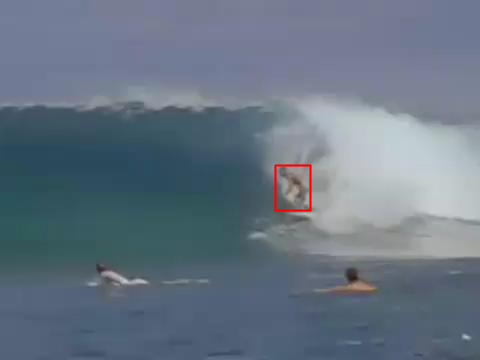
\includegraphics[width=0.9\textwidth]{surfer_marked}
                \caption{Initial frame: The surfer location is known.}
            \end{figure}
        \end{column}
        \begin{column}{0.5\textwidth}
            \begin{figure}
                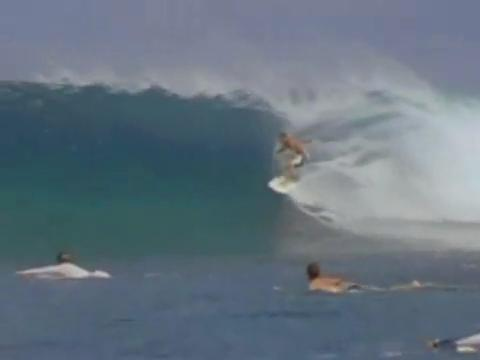
\includegraphics[width=0.9\textwidth]{surfer_unmarked}
                \caption{Subsequent frame: Where is the surfer?}
            \end{figure}
        \end{column}
    \end{columns}
\end{frame}

\begin{frame}
    \frametitle{Tracking can be treated as an object detection problem. \cite{6671560}}
    \begin{columns}[T]
        \begin{column}{0.5\textwidth}
            \begin{description}
                \item [Tracking by detection] Attempt to detect the object in each frame.
                %\item [Adaptive tracking by detection] Update the classifier online.
            \end{description}
            \begin{itemize}
                \item Transform a tracking problem into an object detection problem.
                \item Can use prior knowledge to assist the detection.
                \item For example, in the previous frame, the object was here. In this frame, it's
                    unlikely to be way over there.
            \end{itemize}
        \end{column}
        \begin{column}{0.5\textwidth}
            \begin{itemize}
                \item The algorithm operates on frame \(f_t\), for \(t \in \{1, 2, ..., T\}\).
                \item Sample \(f_t\) around position \(\vec{p}_{t-1}\).
                \item Extract features \(\vec{x}_i\) for each sample.
                \item Input features to a classifier.
                \item Classifier determines which feature corresponds to the tracked object.
                \item Determine new position \(\vec{p}_t\).
                \item Retrain the classifier with new features. \alert{optional}
            \end{itemize}
        \end{column}
    \end{columns}
\end{frame}
